
\section{\sampleclean Estimation}\label{sec:sampleclean}
In this section, we present the \sampleclean estimation approach.
\sampleclean takes a sample of data as input, applies a data cleaning technique to the sample, runs an aggregate query directly on the clean sample,
and returns a result with a confidence interval.

\subsection{Sample Estimates}\label{subsec:resultestimation}
We will first introduce the estimation setting without data errors and explain some results about estimates from sampled data.
We start with the table of $N$ tuples which we call $P$, the \emph{population}.
From $P$, we sample a subset $S$ of size $K$ uniformly; that is, every tuple is sampled with equal probability.
In this setting, we have two problems: (1) Estimate an aggregate query result on the sample $S$; (2) Quantify the uncertainty of the query result.

Consider a simpler problem; suppose we want to estimate the \mean value of $P$.
We can calculate the \mean of $S$ and the Central Limit Theorem (CLT) states that these estimates follow a normal distribution:
\begin{equation}\small
N(\mean(P),\frac{var(P)}{K})
\end{equation}
Since the estimate is normally distributed, we can define a confidence interval parametrized by $\lambda$ (e.g., 95\% indicates $\lambda=1.96$)\footnote{\scriptsize When estimating means of finite population there is a finite population correction factor of $FPC=\frac{N-K}{N-1}$ which scales the confidence interval.}.
\begin{equation}\small
\mean(S) \pm \lambda \sqrt{\frac{var(S)}{K}}.
\end{equation}
This interval has two interpretations: (1) if we re-compute the \mean value on another random sample, the result will be within the confidence interval with the specified probability, and (2)
the true value $\mean(P)$ is within the confidence interval with the specified probability.
Furthermore, we call this estimate \emph{unbiased} since the expected value of the estimate is equal to the true value.

Our primary focus is answering \avgfunc, \countfunc, and \sumfunc queries with predicates\footnote{\scriptsize Group-by queries can be implemented by adding group-by keys into predicates.} (see~\cite{saqpfull} for other queries).
We can estimate these queries by re-formulating them as \mean value calculations.
We first define some notation:
\begin{itemize}\vspace{-.5em}
\item $f(\cdot)$: a function representing any of the supported aggregate queries with a predicate.
\item \Predicate{t}: the predicate of the aggregate query, where \Predicate{t} = 1 or 0 denotes $t$ satisfies or dissatisfies the predicate, respectively.
\item $K$: the number of tuples in the sample.
\item $K_{\pred}$: the number of tuples that satisfy the predicate in the sample.
\item $t[a]$: the aggregation-attribute value. If it is clear from the context that $t$ refers to an attribute value rather than a tuple, we will omit `$[a]$' for brevity.

\end{itemize}
We can reformulate all of the queries as calculating a \mean value so we can estimate their confidence intervals with the CLT:
\begin{equation}\label{eq:general-func}\small
f(S) = \frac{1}{K} \sum_{t \in S} \saqpfunc(t)
\end{equation}
where $\saqpfunc(\cdot)$ expresses all of the necessary scaling to translate the query into a \mean value calculation:
\begin{itemize}\vspace{-.5em}
\item \countfunc: $\saqpfunc(t) = \Predicate{t} \cdot N$\vspace{-.5em}
\item \sumfunc: ~\, $\saqpfunc(t) = \Predicate{t} \cdot N \cdot t[a]$\vspace{-.5em}
\item \avgfunc: ~\, $\saqpfunc(t) = \Predicate{t} \cdot \frac{K}{K_{\pred}}  \cdot t[a] $ 
\end{itemize}
For example, the \avgfunc query is estimated from the sample as:
\begin{equation}
\avgfunc(S) = \frac{1}{K_{pred}}  \sum_{t \in S} \Predicaten{t} \cdot t[a],
\end{equation}
which computes the average value of the tuples that satisfy the predicate in the sample. In order to represent $\avgfunc(S)$ in the form of Equation~\ref{eq:general-func}, we rewrite it to the following equivalent Equation:  
\begin{equation}
\avgfunc(S) = \frac{1}{K}  \sum_{t \in S} \Predicaten{t} \cdot \frac{K}{K_{\pred}}  \cdot t[a].
\end{equation}
Therefore, we have $\saqpfunc(t) = \Predicate{t} \cdot \frac{K}{K_{\pred}}  \cdot t[a] $ for the \avgfunc query.


\iffalse
A key feature of this formulation is the case statement, \Predicate{t}, where tuples that do not satisfy the predicate set the entire term for that tuple by 0. 
It is important to note is that $f(S)$ is defined as the average of $\saqpfunc(\cdot)$ over all tuples including the 0 values, not just the ones that satisfy the predicate.
It will be clear in the subsequent sections that it is convenient to define $f(S)$ in this way to handle condition errors.
However, we need to be careful about scaling factors for each of the queries.

For the \countfunc query, we calculate the average value of \Predicate{t} over all tuples and scale that by the dataset size N.
In other words, this calculates the fraction of tuples that satisfy the predicate, and then multiplies that by the size of the dataset.
Similarly, for the \sumfunc query, we can extend this by multiplying \Predicate{t} by the value of the tuple.
Consequently, we calculate an average value (including 0's for the tuples that don't satisfy the predicate) and we can scale this by the dataset size N.

The \avgfunc query needs a more complex scaling factor.
Since we are interested in the \avgfunc of all the tuples that satisfy the predicate, we have to calculate: 
\begin{equation}
\frac{1}{K_{pred}}  \sum_{t \in S} \Predicaten{t} \cdot t[a]
\end{equation}
However, our formulation of $f(S)$ uses $\frac{1}{K}$ not $\frac{1}{K_{pred}}$.
We accordingly have to rescale by $\frac{K}{K_{\pred}}$ in \saqpfunc(t).
Intuitively, if we include the 0 values from where \Predicate{t} is false in our average, this will lead to an underestimate of the true average.
So, we need to compensate by a factor of $\frac{K}{K_{\pred}}$.
\fi
\subsection{Unbiased Estimation with Data Errors}
If we ignore data errors, the estimates described in the previous section are unbiased.
Suppose $P_{\clean}$ is the corresponding clean population for the dirty data population $P$.
We are interested in estimating an aggregate query on $P_{\clean}$.
However, since we do not have the clean data, we cannot directly sample from $P_{\clean}$.
We must draw our sample from the dirty data $P$ and then clean the sample.

The key question is whether running an aggregate query on the cleaned sample is equivalent to computing the query result on a sample directly drawn from the clean data.
When this is true, our estimate is unbiased, and we can derive confidence intervals using the CLT.
In the following section, we explore this question on different types of data errors.
Our goal is to define a new function $\saqpplusfunc(\cdot)$, an analog to $\saqpfunc(\cdot)$, that corrects attribute values and re-scales to ensures that the estimate remains unbiased.

Recall, that we model three types of errors: value error, condition error, and duplication error.
To correct the errors, we can define two data cleaning primitive functions:
\begin{itemize}\vspace{-.5em}
\item \Correct{t}: for the tuple t return a tuple with correct attribute values\vspace{-.5em}
\item \Dedup{t}{P}: for the tuple t return the number of times that the tuple appears in the population~$P$ 
\end{itemize}


\subsubsection{Value and Condition Errors}
Both value and condition errors are caused by incorrect attribute values of the dirty data.
These errors do not affect the size of the population, i.e., $|P| = |P_{\clean}|$.
Furthermore, correcting a value or condition error only affects an individual tuple.
Consequently, if we apply the $\saqpfunc(\cdot)$ to the corrected tuple, we still preserve the uniform sampling properties of the sample, $S$.
In other words, the probability that a given tuple is sampled is not changed by our correction of value and condition errors, thus we define $\saqpplusfunc(t)$ as:
\begin{equation}\small
\saqpplusfunc(t) = \saqpfunc \left( \Correct{t} \right).
\end{equation}

Note that the $\saqpfunc(\cdot)$ for an \avgfunc query is dependent on the parameter $K_{\pred}$. 
If we correct values in the predicate attributes, we need to recompute $K_{\pred}$ in the cleaned sample.

\subsubsection{Duplication Error}\label{subsec:challenges}
Since duplication errors affect multiple tuples and the size of $P_{\clean}$ is different from the size of $P$, they do affect the uniformity of the sampling.
The following example illustrates the consequences of duplication errors:
\begin{example}
Consider a population $P = \{t_1, t_2, t'_2\}$ with two distinct tuples, $t_1$ and $t_2$ (=$t'_2$).
If we draw samples of size 2 from this population uniformly:
\[ Pr(\{t_1, t_2\})=\frac{1}{3},\ Pr(\{t_1, t'_2\})=\frac{1}{3},\ Pr(\{t_2, t'_2\})=\frac{1}{3}. \]
Now, assume $t_1 = 1$ and $t_2 = t_2' = 2$.
The expected \mean value over all random samples is $\frac{1}{3}\cdot\frac{3}{2}+\frac{1}{3}\cdot\frac{3}{2}+\frac{1}{3}\cdot2=\frac{5}{3}$, however the cleaned population is $P_{\clean} = \{t_1, t_2\}$ and its \mean value is actually $\frac{3}{2}$. %Thus, when duplication errors exist, it may be biased to estimate a result based on the cleaned sample.
\end{example}
The duplicated data is more likely to be sampled and thus be over-represented in the estimate of the \mean.
We can address this with a weighted mean to reduce the effects of this over-representation.
Furthermore, we can incorporate this weighting into $\saqpplusfunc(\cdot)$.

Specifically, if a tuple $t$ is duplicated $m=\Dedup{t}{P}$ times, then it is $m$ times more likely to be sampled, and we should down weight it with a $\frac{1}{m}$ factor compared to the other tuples in the sample.
We formalize this intuition with the following lemma:
\begin{lemma}\label{lem:derror}
Let $P$ be a population with duplicated tuples. % and $P_{unique}$ be the set of unique tuples.
Let $S \subseteq P$ be a uniform sample of size $K$.
For each $t_{i}\in S$, let $m_i$ denote its number of duplicates in $P$.
 (1) For \sumfunc and \countfunc queries, applying $\saqpplusfunc(t_i)=\frac{\saqpfunc(t_i)}{m_i}$ yields an unbiased estimate;
(2) For an \avgfunc query, the result has to be scaled by the duplication rate $d=\frac{K}{K'}$,
where $K'=\sum_i\frac{1}{m_i}$, so using $\saqpplusfunc(t_i)=d\cdot\frac{\saqpfunc(t_i)}{m_i}$ yields an unbiased estimate.
\end{lemma}

\begin{proof}[sketch] We can interpret the population as a discrete probability distribution, and the sample as drawing $K$ elements from this distribution.
Since some elements are duplicated there is an increased probability of drawing these elements.
We reduce these effects by re-weighting the samples, which can be thought of as drawing fractional samples (i.e., if we sample an element which is duplicated twice, we cancel it out by treating it as sampling only half an element).
As a result, while we may draw $K$ total samples, the total number of fractional samples drawn (sum of the weights) $K'$,
may be different, so we have to scale the result accordingly. See~\cite{saqpfull} for a detailed proof.
\end{proof}
We apply this lemma to the following example:
\begin{example}\label{exa:derror}
Consider the dirty data in Figure~\ref{fig:example}, $P = \{t_1, t_2, \cdots, t_{10000}\}$, and the sample data, $\Sset = \{t_1, t_2, t_3, t_4,$ $t_5, t_6, t_7\}$. In this example, we assume the data only has duplication error, and our goal is to estimate the average citation count of all the papers in the data. 

Firstly, we compute the duplication rate of the sample: 
\[\frac{K}{\sum_{t\in S} \frac{1}{\Dedup{t}{P}}} = \frac{7}{\frac{1}{2}+\frac{1}{1}+\frac{1}{2}+\frac{1}{1}+\frac{1}{1}+\frac{1}{1}+\frac{1}{3}} = 1.31\]

Then, we apply $\saqpplusfunc(\cdot)$ to each paper $t\in \Sset$. Specifically, we divide its citation count by the number of duplicates and then multiple it by the duplication rate, i.e., $\saqpplusfunc(S) = \{\frac{1.31\cdot 18}{2}, \frac{1.31\cdot1569}{1}, \frac{1.31\cdot298}{2}, \cdots , \frac{1.31\cdot687}{3}\}$. For example, the first paper's citation count is 18 and it has two duplicates, thus we have $\saqpplusfunc(t_1) = \frac{1.31\cdot 18}{2}$. 


Finally, we estimate the average citation count as the \mean of $\saqpplusfunc(S)$.

%Firstly, for each paper $t\in \Pset$, we divide its citation count by the number of duplicates, and obtain a set of corrected citation counts for the sample data, i.e., $\saqpplusfunc(S) = \{\frac{18}{2}, \frac{1569}{1}, \frac{298}{2}, \frac{106}{1}, \frac{107}{1}, \frac{1}{1}, \frac{687}{3}\}$.
%Then we take the weighted average of the sample, which is $\frac{1}{7}\cdot (\frac{18}{2}+\frac{1569}{1}+\frac{298}{2}+\frac{106}{1}+\frac{107}{1}+\frac{1}{1}+ \frac{687}{3}) = 310$.


%Therefore, based on Lemma~\ref{lem:derror}, we can estimate the average citation count, i.e., $1.31*310 = 406.1$.
\end{example}

\subsubsection{Combinations of Errors}\label{subsec:comb-challenge}
We can also address data with combinations of errors (e.g., duplicated tuples that also have incorrect values).
Value and condition errors affect a tuple's values.
Duplication errors affect a tuple's sampling probability.
The two classes of errors affect the tuple in different ways, and consequently, we define a single function $\saqpplusfunc(\cdot)$ which can correct for all three error types:


\begin{itemize}\vspace{-.5em}
\item \countfunc: $\saqpplusfunc(t) = \frac{\saqpfunc(\Correct{t})}{\Dedup{t}{P}}$\vspace{-.5em}
\item \sumfunc: ~\, $\saqpplusfunc(t) =\frac{\saqpfunc(\Correct{t})}{\Dedup{t}{P}}$\vspace{-.5em}
\item \avgfunc: ~\, $\saqpplusfunc(t) = d\cdot\frac{\saqpfunc(\Correct{t})}{\Dedup{t}{P}}$ 
\end{itemize}

We plug $\saqpfunc(\cdot)$ (as described in Section~\ref{subsec:resultestimation}) into the above equations, and obtain a more detailed form of $\saqpplusfunc(t)$ as shown in Table~\ref{tbl:transform-new}.
%Let $N$ be the total size of the dataset (including duplicates), $K$ be the size of the sample (including duplicates), $K_{pred}$ be the number of tuples in the sample that satisfy the predicate (including duplicates), and $d$ be the duplication rate estimated from the sample. 
%We get the following transformations:
%For more details about the composability of these functions, see~\cite{saqpfull}.

\iffalse
\begin{table}[htup]\vspace{-1em}
\label{tbl:transform}
\scriptsize
\caption{$\saqpplusfunc(\cdot)$ for \sumfunc, \countfunc, and \avgfunc}
\centering 
\begin{tabular}{l l}
\hline\hline
Query & $\saqpplusfunc(\cdot)$\\
\hline  % inserts single horizontal line
\vspace{.5em}
$\avgfunc$ & $\frac{d\cdot\saqpfunc(\Correct{t})}{\Dedup{t}{P}}
$ \\\vspace{.5em} % inserting body of the table
$\sumfunc$ & $ \frac{\saqpfunc(\Correct{t})}{\Dedup{t}{P}}
$ \\\vspace{.5em}
$\countfunc$ & $
		\frac{\saqpfunc(\Correct{t})}{\Dedup{t}{P}}
$ \\ [1ex] % [1ex] adds vertical space
\hline %inserts single line
\end{tabular}
\end{table}
\fi


\begin{table}[htup]\vspace{-1em}

\small
\caption{$\saqpplusfunc(\cdot)$ for \countfunc, \sumfunc, and \avgfunc. Note that $N$ is the total size of dirty data (including duplicates).}
\centering 
\begin{tabular}{l l}
\hline\hline
Query & $\saqpplusfunc(\cdot)$\\
\hline  % inserts single horizontal line
\vspace{.5em}
$\countfunc$ & $
		\Predicatec{t}\cdot N\cdot\frac{1}{\Dedup{t}{P}}
$ \\\vspace{.5em} % inserting body of the table
$\sumfunc$ & $
		\Predicatec{t}\cdot N\cdot\frac{\Correct{t}[a]}{\Dedup{t}{P}}
$ \\\vspace{.5em}
$\avgfunc$ & $
		\Predicatec{t}\cdot \frac{dK}{K_{\pred}}\cdot\frac{\Correct{t}[a]}{\Dedup{t}{P}}
$ \\ [1ex] % [1ex] adds vertical space
\hline %inserts single line 
\label{tbl:transform-new}
\end{tabular}\vspace{-2em}
\end{table}


\vspace{.5em}
{\noindent \bf \sampleclean Estimation:}
We can now formulate the \sampleclean estimation procedure, as follows:

\begin{enumerate}
\item Given a sample $S$ and an aggregation function $f(\cdot)$\vspace{-.5em}
\item Apply $\saqpplusfunc(\cdot)$ to each $t_i \in S$ and call the resulting set $\saqpplusfunc(S)$\vspace{-.5em}
\item Calculate the mean $\mu_c$, and the variance $\sigma_c^2$ of $\saqpplusfunc(S)$\vspace{-.5em}
\item Return $\mu_c \pm \lambda \sqrt{\frac{\sigma_c^2}{K}}$\vspace{-.5em}
\end{enumerate}

To summarize, we state that the \sampleclean approach gives an unbiased estimate:

\begin{theorem}\label{thm:sampleclean}
Given an aggregation function $f$ and a population $P$,
where there are three types of errors: value, condition, and duplication.
Let S be a uniform sample $S \subseteq P$ of size $K$.
Let $\saqpplusfunc(S)$ be the set of tuples where $\saqpplusfunc(\cdot)$ is applied to every tuple.
Then the estimate on this sample is given by:
\[ \mean \left( \saqpplusfunc(S) \right) = \frac{1}{K}\sum_{t\in S} \saqpplusfunc(t) \]
The estimate is an unbiased estimate of $f(P_{\clean})$.
\end{theorem}
\begin{proof}[sketch]
We need to show that the aggregation $\saqpplusfunc(S)$ is equivalent to the aggregation $\saqpfunc(S_{\clean})$.
Lemma~\ref{lem:derror} shows that this is true for duplication errors.
We further argued that with value errors and condition errors $\saqpplusfunc(S) = \saqpfunc(S_{\clean})$.
Finally, since duplication error correction and value/condition correction can be composed this is true.
As the \mean of a uniform random sample of $P_{\clean}$, this is an unbiased estimate.
See~\cite{saqpfull} for a detailed proof.
\end{proof}

%For each paper $t\in S$, if $t$ is removed from $S$ (i.e. $\Remove{t}{P}$ = True), we set $\phi_f(t) = 0$; otherwise, we first correct its citation number (i.e. \Correct{t}), and then divide the correct citation number by the number of duplicates (i.e., |\Dedup{t}{P}|), and finally obtain its transformed value $\phi_f(t)=\frac{d}{r}\cdot\frac{\Correct{t}}{|\Dedup{t}{P}|}$.
Consider the following end-to-end numerical example with \sampleclean:

\begin{example}\label{exa:sampleclean}
Consider the sample data and the cleaning results in Figure~\ref{fig:sample}, and assume the data may involve three types of errors.
To estimate the query result, we need to map each $t \in S$ to a new value $\saqpplusfunc(t)$.
Since the sample contains seven papers, and $t_4$ and $t_7$ do not satisfy the predicate, the scaling for predicates is $\frac{K}{K_{\pred}} = \frac{7}{5}=1.40$.
As shown in Example~\ref{exa:derror}, the duplication rate is $d = 1.31$.
After applying $\saqpplusfunc(\cdot)$ for \avgfunc query in Table~\ref{tbl:transform-new} to each sampled paper, we obtain the transformed sample data of $\saqpplusfunc(S) = \{133,\, 2895,\, 275,\, 0,\, 197,\, 63,\, 0\}$.
For example, since $t_1$ satisfies the predicate, and its correct citation count is 144 and the number of duplicates is 2, we have $\saqpplusfunc(t_1) = 1.31\cdot 1.40 \cdot\frac{144}{2} = 133$.
Similarly, as $t_4$ does not satisfy the predicate, we have $\saqpplusfunc(t_4) = 0$. 
We calculate the \mean $\mu_c$ and the variance $\sigma_c^2$ of $\saqpplusfunc(S)$, and return $\mu_c \pm \lambda \sqrt{\frac{\sigma_c^2}{K}}$ as the estimated average citation count, where $\lambda$ is a constant value derived from the user-specified confidence probability.
\end{example}

\begin{figure}[t]\vspace{-1em}
\centering
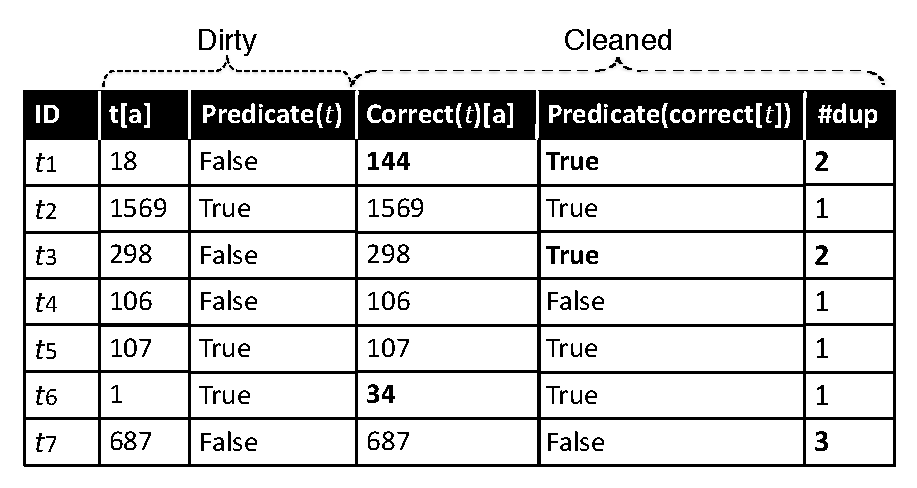
\includegraphics[scale=0.45]{figs/sample.pdf}\vspace{-1em}
\caption{The cleaning results for the sample $\Sset = \{t_1, t_2, t_3, t_4, t_5, t_6, t_7\}$  w.r.t ``SELECT \textsf{AVG}(citation\_count) FROM papers WHERE pub\_year>2000". The values in bold font indicate the changed values after data cleaning.}\vspace{-.5em}
\label{fig:sample}\vspace{-.5em}
\end{figure}

\vspace{.5em}
{\noindent \bf Remarks.} % There are a few additional remarks about \sampleclean. 
%We have mentioned that the \avgfunc query is affected by scaling since its result has to be scaled by the size of the sample.
(1) For an \avgfunc query, we can achieve tighter confidence intervals by skipping the tuples that dissatisfy the predicate instead of considering them as 0 values.
The reason for this is that the \avgfunc query has a scaling factor $r=\frac{K}{K_{\pred}}$, which is a random variable itself.
The confidence intervals we present incorporate the additional variance of~$r$, but due to the skipping we can get estimates not affected by that variance. (2) Algorithmically, we contrast \sampleclean from \saqp with $\saqpplusfunc(\cdot)$ vs. $\saqpfunc(\cdot)$, which makes it very convenient to implement \sampleclean in an existing \saqp system.
%This is particularly convenient for implementation since, if we know the query, we can simply transform the data prior to passing it to an existing \saqp framework.

%The method can obtain unbiased query results along with quality guarantees from the cleaned sample.
%We first introduce a basic theory of sample-based result estimation in Section~\ref{subsec:resultestimation}, and then 
%discuss the new challenges posed by data errors in Section~\ref{subsec:challenges}. We addresses these challenges and present the \sampleclean algorithm in Sections~\ref{subsec:dup-challenge} and~\ref{subsec:comb-challenge}.
%Note that there are other ways (e.g., bootstrapping~\cite{hinkley1988bootstrap}) to compute confidence intervals.
%In principle, we can use other confidence interval techniques, and we illustrates how to use bootstrapping for queries that do not have convenient analytic confidence intervals in~\cite{saqpfull}.


%\begin{lemma}\label{lem:derror}
%Let $P$ be a population with $N$ data tuples, and $P^{c}$ the cleaned population  with $N'$ unique data tuples. For each $p_{i}\in P$, let $m_i$ denote its number of duplicates in $P$ and let $\frac{p_{i}}{m_{i}}$
%represent a data tuple where the aggregation-attribute value is 
%divided by $m_{i}$. Then for the set $\hat{P}^{c}=\{\frac{p_{1}}{m_{1}},\frac{p_{2}}{m_{2}},...,\frac{p_{N}}{m_{N}}\}$,
%the mean value (denoted by $\mathbb{E}(\cdot)$) of the set $\hat{P}^{c}$ is:
%\[
%\mathbb{E}(P^{c})=d\cdot \mathbb{E}(\hat{P}^{c}) 
%\]
%where $d$ is the duplication ratio $\frac{N}{\sum_{i}^{N}\frac{1}{m_{i}}}=\frac{N}{N'}$.
%\end{lemma}
%\begin{proof}[sketch] (See Appendix) We can treat a population as a discrete probability distribution over the values of its aggregation attribute.
%Since $\mathbb{E}(X):=\sum_i iPr(X==i)$, if an attribute with the value i has been duplicated $m$ times then $Pr(X==i)$ is $m$ higher so down weighting
%those attributes by a factor of $m$ compensates for the increase.
%\end{proof}\vspace{-1em}

%As important consequence of this lemma is that we can extend this reasoning to samples and obtain an unbiased estimate.

%\subsection{Combinations of Errors}\label{subsec:comb-challenge}
%In our problem formulation, we discussed two other forms of errors: aggregation errors and predicate errors.
%These can similarly be addressed through design of $\phi^{*}_f(\cdot)$.

%With aggregation errors, the intuitive transformation works where we set an incorrect value to its correct value.
%Since these errors only affect single tuples, the estimate on the transformed data is still unbiased and it is functionally similar to sampling from a data where all the tuples have cleaned aggregation-attribute values.

%Predicate errors are a little bit more complex since they not only affect the value of an aggregation, they also have effects on the size of the sample.
%However, we can use a similar trick as the previous section where rather than removing a tuple that does not satisfy the query predicate, we can set its value to zero.
%Since all of our queries follow additive forms, this means that the tuple does not contribute to the result.

%Similar to scaling problem with duplication errors, the \avgfunc will be off by a proportionality constant $r$, which is the fraction of tuples that satisfy the query.
%We accordingly use the estimate $\hat{r}$, the fraction of tuples in the sample that satisfy the predicate, to maintain the correct scaling. 

%Based on this design of $\phi^{*}_f(\cdot)$, we propose the following:

%\begin{lemma}\label{lem:comp}
%Given an aggregation function $f$,
%let $\phi^{*}_{f(1)}$ be the transformation
%that estimates unbiasedly under duplication
%errors. Let $\phi^*_{f(2)}$ be unbiased
%under predicate errors, and $\phi^*_{f(3)}$
%be unbiased under aggregation errors.
%We can define a composed function $\phi^*_f(\cdot) = \phi^*_{f(2)}(\phi^*_{f(1)}(\phi^*_{f(3)}(\cdot)))$,
%that is unbiased under all three errors.
%\end{lemma}
%\begin{proof}[sketch] 
%We can re-define clean estimation in stages: (1) estimate the function unbiasedly if aggregation errors were the only problem,
%(2) given data that is free of aggregation errors, we fix duplication errors, (3) finally, we remove tuples that do not satisfy the predicate. In this order of operations, the functions are
%composable. See~\cite{saqpfull} for a detailed proof.
%\end{proof}

%As a result, we have a single choice of $\phi^*_f(\cdot)$ as shown in Table~\ref{tbl:transform} that addresses our three types of data errors.
%\subsection{SampleClean Algorithm}
